\documentclass[]{article}

\usepackage[]{struktex}
\usepackage{graphicx}
\usepackage{lmodern}
\usepackage{svg}

\usepackage[utf8]{inputenc}
\usepackage[T1]{fontenc}
\usepackage[ngerman]{babel}
\usepackage[left=2cm, right=2cm, top=2cm, bottom=2cm, bindingoffset=8mm, includehead, includefoot]{geometry}

% subfigures
\usepackage{caption}
\usepackage{subcaption}

\usepackage{amsfonts}
\usepackage{amssymb}
\usepackage{amsmath}

% Nummerierung mit Alpabet
\usepackage{enumitem}

% paragraph wird wie subsubsection dargestellt und in Inhaltsverzeichnis aufgenommen
\usepackage{titlesec}
\setcounter{secnumdepth}{4}
\setcounter{tocdepth}{4}

\titleformat{\paragraph}
{\normalfont\normalsize\bfseries}{\theparagraph}{1em}{}
\titlespacing*{\paragraph}
{0pt}{3.25ex plus 1ex minus .2ex}{1.5ex plus .2ex}

%opening
\title{Final Task EIB3 WS24|25}
\author{Niklas Bachmann \\ Manuel König}

\begin{document}
	
	\maketitle
	%\tableofcontents
	
	\section{Schematics}
		\begin{figure}[htp]
				\centering
				%\includesvg{Proj_scheme.svg}
				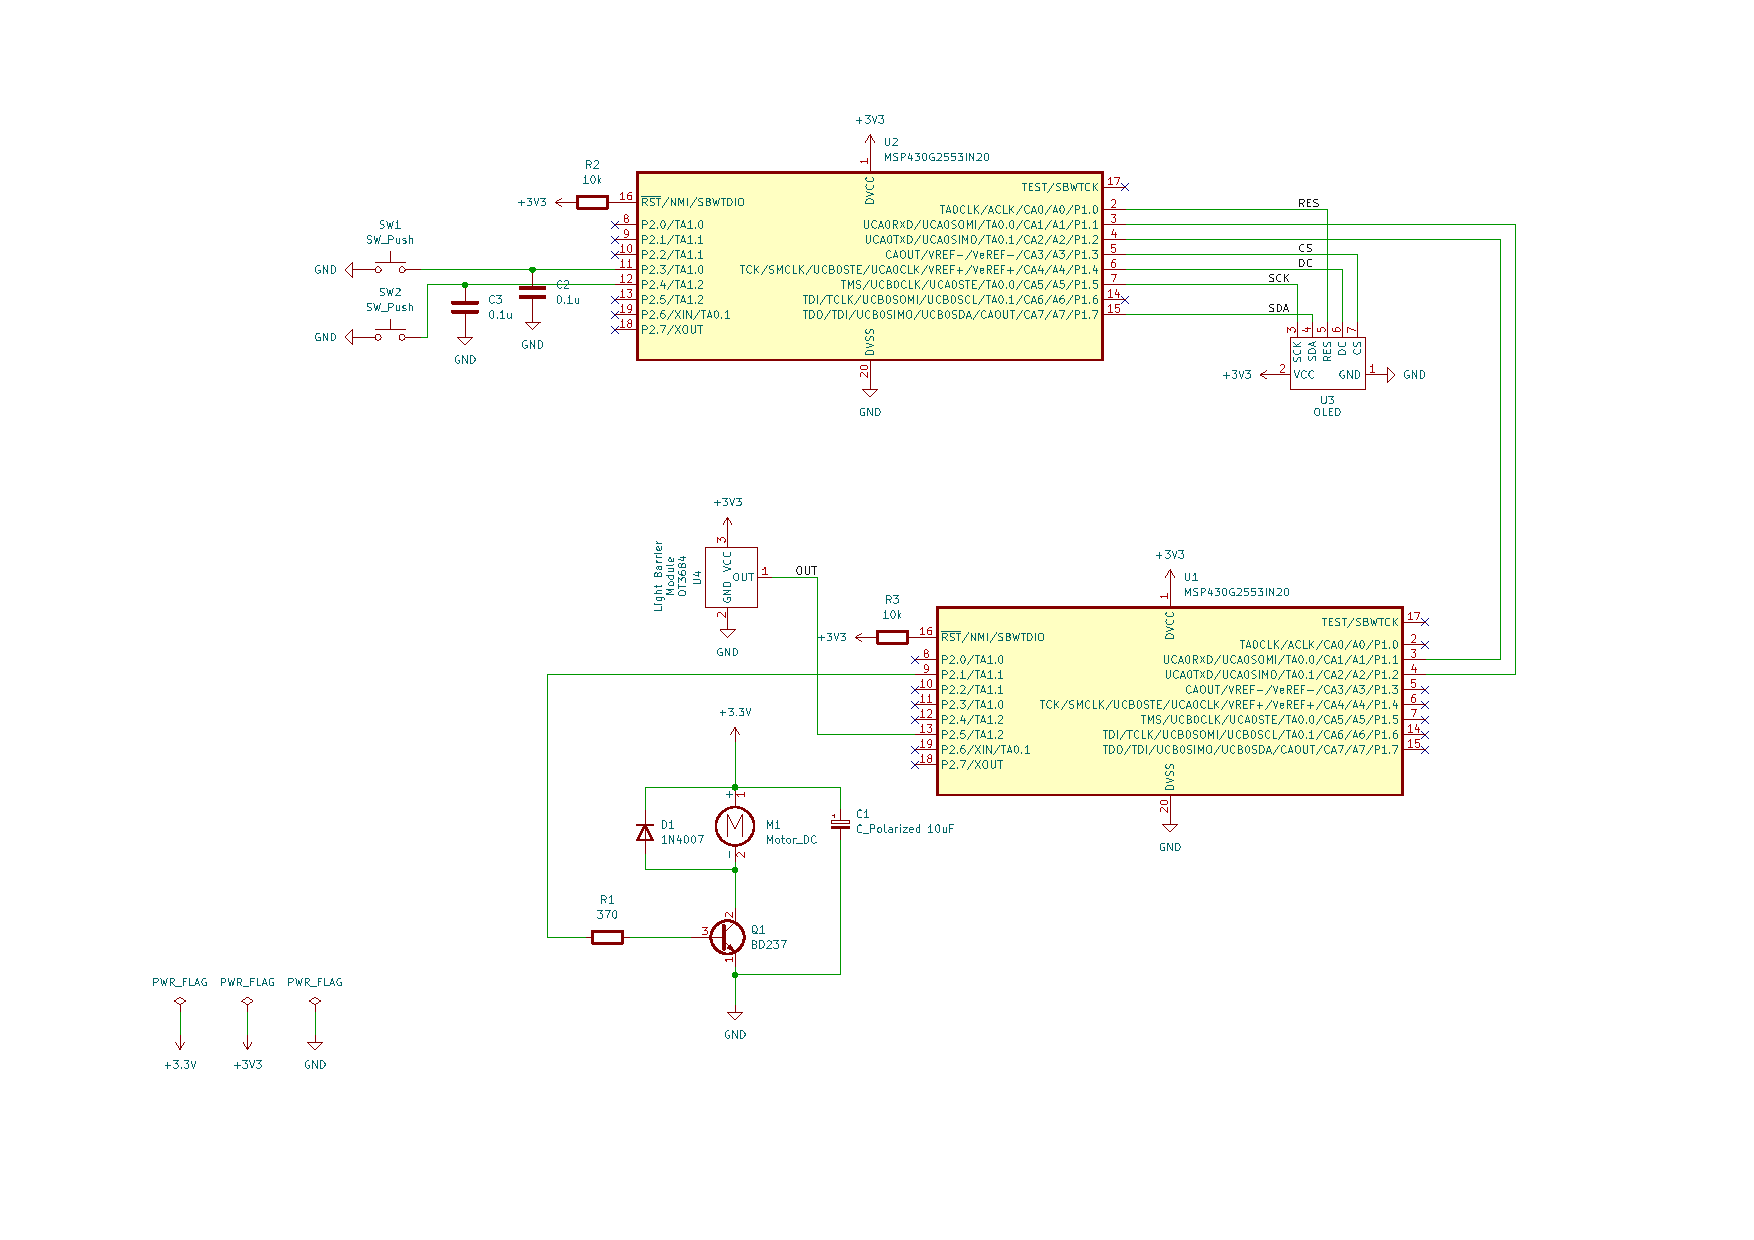
\includegraphics[width=17cm]{Proj_scheme} %[width=9cm, trim=0 2cm 0 0, clip = true]
				\caption{Project scheme}
		\end{figure}
	
	\newpage
	\section{Structograms}

	\begin{figure}[htp]
		\centering
		\begin{struktogramm}(160,100)
			\sub{pressButton}
			\sub{updateDisplay}
			\sub{encodeMotorSpeed}
			\sub{sendMotorSpeed}
			\sub{receiveMotorSpeed}
			\assign{setFlag {ABCDZ}}
			\ifthenelse{4}{1}{ABC Flag}{\sTrue}{\sFalse}
				\sub{atoi convert to integer}
				\ifthenelse{3}{1}{if atoi == len}{\sTrue}{\sFalse}
					\assign{move result to targetSpeed}
					\change
				\ifend
				
			% wie  wir Vollständigkeit des Strings bestimmt
			% Flag in ISR
			% if flag : atoi
			% if len == 5 : move 
				\change
			\ifend
			\sub{updatePID}
			\sub{getActualMotorSpeed}
			\sub{sendActualMotorSpeed}
			\sub{updateDisplay}

		\end{struktogramm}
	\end{figure}
	
\end{document}
